%!TEX root = bachelor.tex
\chapter{Analyse}
\label{ch:analysis}
\todo{analyse einleitung schreiben}
In diesem Kapitel...

Zunächst werden die beiden Verfahren zur Entzerrung gegenübergestellt\todo{ändern}. Anschließend untersuchen wir verschiedene Einflüsse auf der Qualität der Entzerrung, woraufhin wir die Laufzeit ermitteln. 
Zum Schluss Ransac...

Die Laufzeitanalysen wurden auf einem Raspberry Pi 2 Model B durchgeführt mit folgenden Eigenschaften:
\begin{itemize}
	\item 900MHz ARM Cortex-A7 CPU
	\item 1GB RAM
	\item GCC-4.9.2
	\item Opencv 2.4.13
\end{itemize}


\section{Vergleich Vorwärtsentfaltung und Rückwärtsentfaltung}
Untersucht man die interpolierten Weltkoordinaten bei der Vorwärtsentfaltung, stellt man fest, dass die Oberfläche des Kegels,  wie in Abbildung \ref{fig:3DInterpol} zu sehen, eckig scheint. Zur Veranschaulichung wird hierbei nur ein Bruchteil der interpolierten Werte dargestellt. Zwischen den Samples auf einer Kreislinie sollten die interpolierte Positionen nach außen gewölbt sein, da ein Kegel rund ist. Da wir jedoch interpolieren und nicht extrapolieren, gehen die Werte nie über die zur Interpolation genutzten Werte hinaus. Konkreter kann eine interpolierte Position keine größeren oder kleineren $x$- und $y$-Koordinaten erhalten, als die der genutzten Samples. Diese wäre jedoch notwendig, sodass die Rundung des Kegels erhalten bleibt.

\begin{figure}[!htb]
	\centering
	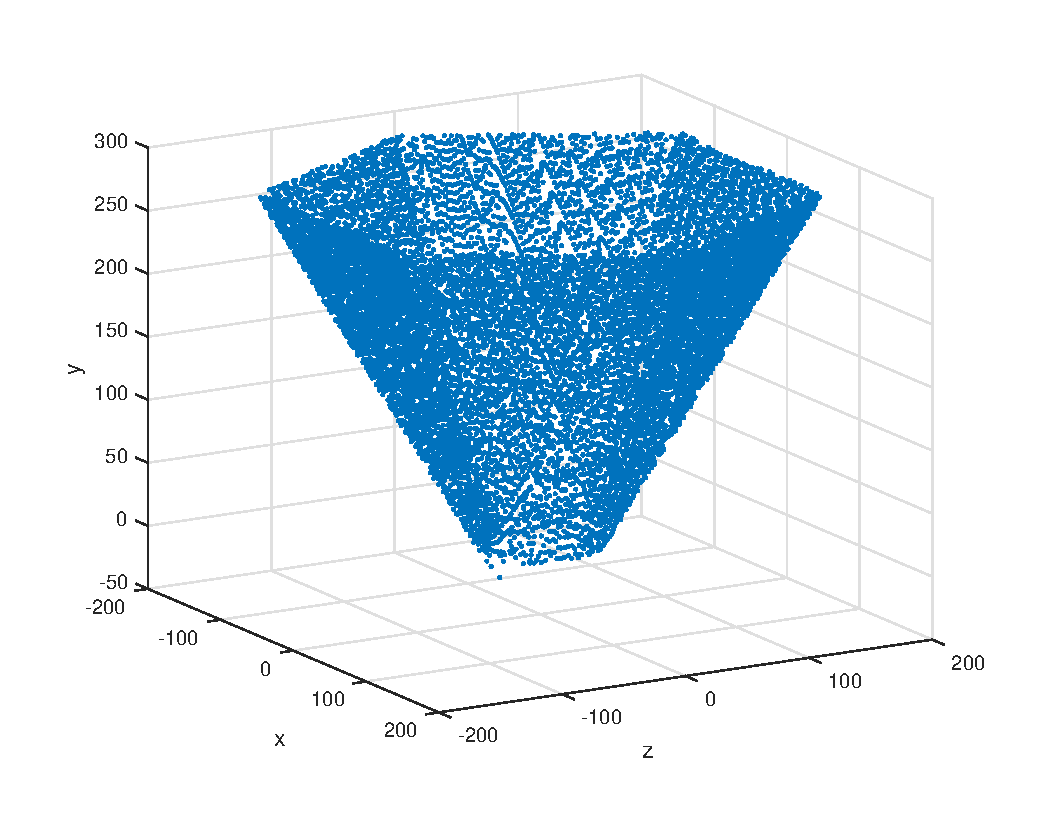
\includegraphics[scale=.7]{images/3d_interpol.eps}
	\caption{interpolierter Kegel}
	\label{fig:3DInterpol}
\end{figure}

\begin{figure}[!htb]
	\centering
	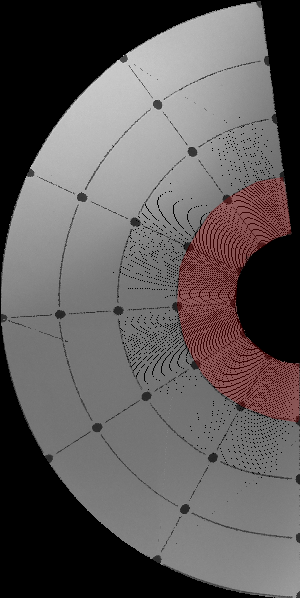
\includegraphics[angle=-90, width=.7\textwidth]{images/coneRaspUnWarpForwardHigh.png}
	\caption{Vorwärtsentfaltung}
	\label{fig:forwardHoles}
\end{figure}

Darüber hinaus zeigt sich ein weiteres Problem nach der Entfaltung. Die Entfaltung geschieht über die Abbildung \ref{eq:coneToLateral}, die in Kapitel \ref{s:cone} konstruiert wurde. 
Damit im entfalteten Bild nicht 1mm einem Pixel entspricht, müssen die erhaltenen Werte skaliert werden. Wir wollen dabei entsprechend einer gewünschten Auflösung der entzerrten Seitenhöhe skalieren. 
Auch schon bei kleineren Skalierungen entstehen auffällige Risse im entfalteten Bild, die in Abbildung \ref{fig:forwardHoles} exemplarisch zu sehen sind. Grund dafür ist, dass jedes Pixel aus dem Ursprungsbild auf eine 2D-Koordinate der Mantelfläche abgebildet wird. Auch nach einer Skalierung handelt es sich bei diesen Werten im Allgemeinen nicht um ganzzahlige Werte. Es entstehen Rundungsfehler. Auch wenn Rundungsfehler nicht entständen, fehlte es auf Grund der starken Stauchung, in den inneren, kleineren Regionen (siehe Abbildung \ref{fig:forwardHoles} in rot) des Ursprungsbild an genügend Bildinformation. Solche Risse, beziehungsweise nicht erreichte Pixel auf dem entfalteten Bild, bezeichnen wir als Defekte. 

Da wir von dem Ursprungsbild aus auf das entfaltete Bild abbilden, ist außerdem eine Interpolation auf dem Ursprungsbild nicht möglich, da wir vorher nicht wissen, wo Defekte entstehen. Man müsste also entweder auf dem resultierendem Bild interpolieren (siehe Kapitel \ref{ch:summary}), oder zu gegebenen Defekten über die Umkehrabbildung auf Pixelkandidaten im Ursprungsbild schließend und dann entsprechend interpolieren. 
Es bietet sich dann jedoch an, direkt die Umkehrabbildung zu nutzen, was die Motivation hinter der Rückwärtsentfaltung ist.

Wir möchten untersuchen wie sich die Anzahl der Defekte bei einer Änderung der Ausgabeauflösung verhält. Diese Beziehung lässt sich in Abbildung \ref{fig:influenceRes} ablesen. 
\begin{figure}[!htb]
	\centering
	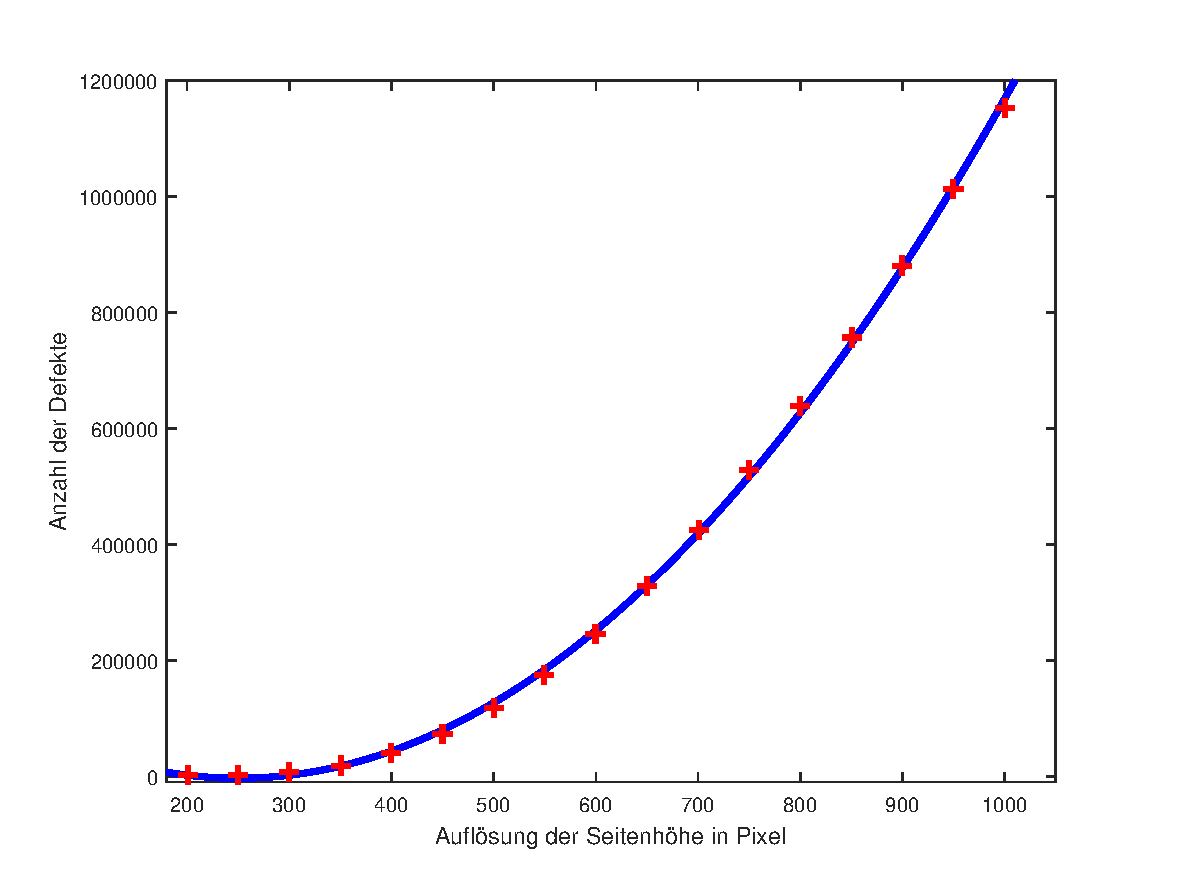
\includegraphics[width=\textwidth]{images/numberOfHoles.eps}
	\caption{Einfluss der Ausgabeauflösung auf die Anzahl der Defekte}
	\label{fig:influenceRes}
\end{figure}

Wie erwartet verhält sich die Anzahl der Defekte quadratisch zur gewählten Ausgabeaufösung. Der Informationsgehalt (Pixelanzahl) des Ursprungsbild bleibt trotz erhöhter Ausgabeauflösung konstant. Wie in Abbildung \ref{fig:sizeOutput} zu sehen, verhält sich die Ausgabeauflösung quadratisch zur Gesamtzahl der Pixel für ein konstantes $\alpha$. Für die Breite $b$ des Ausgabebildes gilt $b = res_S$. 
Die Höhe $h$ setzt sich wie folgt zusammen: $h = res_S + res_S\cdot\cos(2\pi-\alpha) = res_S\cdot(1 + cos(2\pi-\alpha)) = res_S\cdot(1+\cos\alpha)$. Dazu betrachten wir das rechtwinklige Dreieck in der rechten oberen Ecke der Abbildung (in magenta). Die Hypotenuse des Dreiecks beträgt $res_S$ und mit $\beta = 2\pi - \alpha$ ergibt sich für die Ankathete eine Länge von $res_S\cdot\cos(2\pi-\alpha)$. Die Gesamtzahl der Pixel beträgt demnach $b\cdot h = res_S^2(1+\cos(\alpha))$.

\begin{figure}[!htb]
	\centering
	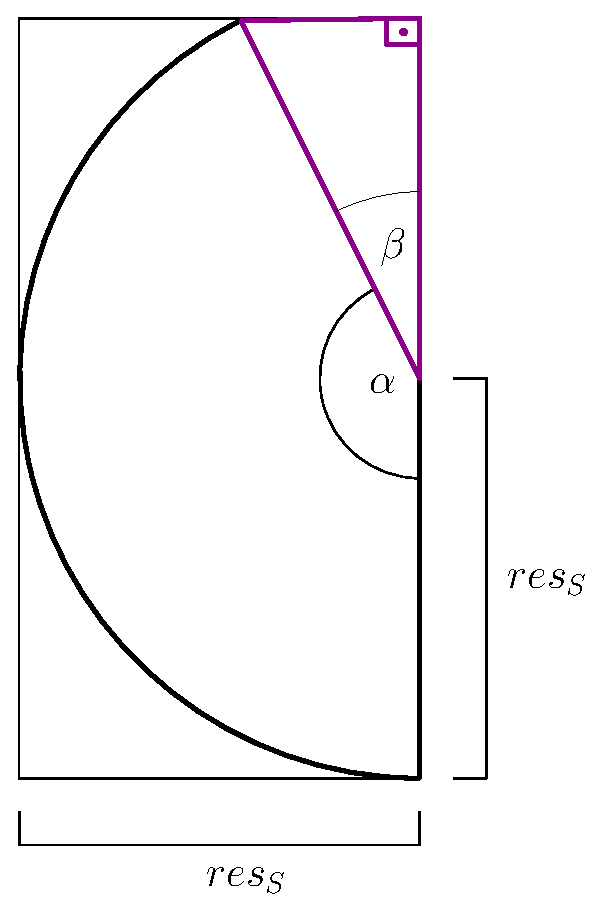
\includegraphics[width=0.3\textwidth]{images/sizeOutput.eps}
	\caption{Größe des Ausgabebildes bei einer Seitenhöhe von $res_S$}
	\label{fig:sizeOutput}
\end{figure}


Obwohl die Laufzeit der Kalibrierung nicht im Vordergrund steht, vergleichen wir die Laufzeit beider Verfahren bei verschiedenen Auflösungen der Seitenhöhe. Da der Großteil des Kalibrierungsprozesses bei beiden Verfahren identisch ist, vergleichen wir nun den Teil, der sich unterscheidet. Das heißt wir messen bei der Vorwärtsentfaltung die Laufzeit für die Interpolation der Weltkoordinaten und die anschließende Abbildung auf die Mantelfläche, und bei der Rückwärtsentfaltung die Laufzeit für die Abbildung auf die Kegelkoordinaten, die Bestimmung der Projektionsmatrix und die anschließende Abbildung auf die Bildkoordinaten, inklusive Interpolation.


Wie in Abbildung \ref{fig:runningTimeComparision} zu sehen, ist der Aufwand bei bei der Vorwärtsentfaltung weitestgehend konstant. Dies da dadurch zu begründen, dass sich die Eingabeauflösung nicht ändert. Der Interpolationsaufwand bleibt gleich und es wird anschließend die gleiche Anzahl Pixel auf die Mantelfläche abgebildet. Nur der Ort der Projektion wird entsprechend der Ausgabeauflösung skaliert. 
Bei der Rückwärtsentfaltung hingegen, wächst der Interpolationsaufwand quadratisch. Wir gehen dort von dem Ausgabebild aus, das quadratisch mit der Auflösung wächst und bilden dort jeden Punkt auf das Ursprungsbild ab. Je mehr Pixel auf dem Ausgabebild, desto häufiger muss interpoliert werden. Bei einer Auflösung der Seitenhöhe von $850$ Pixeln ist die Laufzeit bei beiden Verfahren gleich. 

\begin{figure}[!htb]
	\centering
	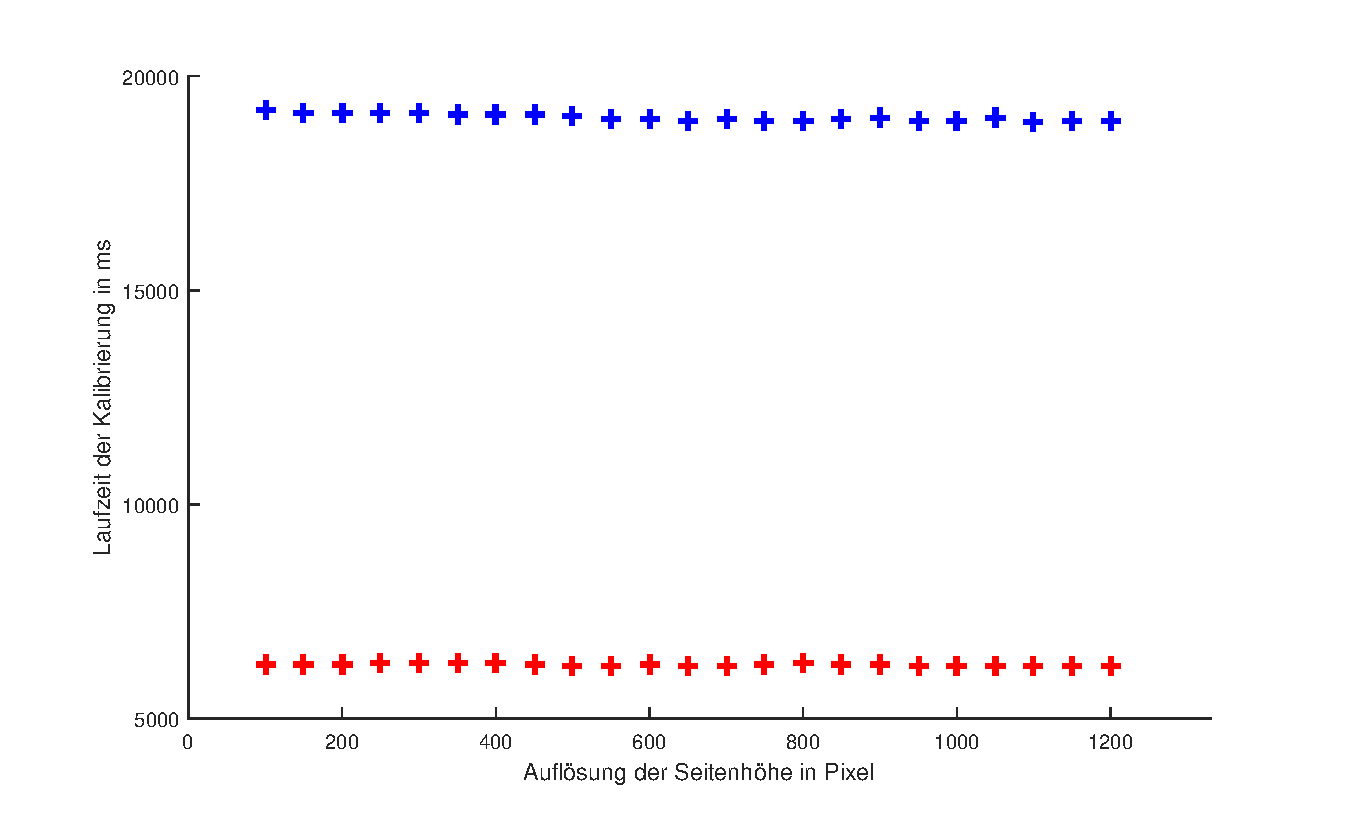
\includegraphics[width=0.9\textwidth]{images/runningTimeCalibration.eps}
	\caption{Laufzeitvergleich zwischen Vorwärtsentfaltung (blau) und Rückwärtsentfaltung (rot)}
	\label{fig:runningTimeComparision}
\end{figure}


\bigskip

Als Reprojektionsfehler einer Abbildung wird die Distanz zwischen einem gemessenem Punkt und einem korrespondierendem (durch die Abbildung) projizierten Punkt bezeichnet. 


Im Falle der Rückwärtsentfaltung sind die gemessenen Punkte die Bildpositionen der Samples im Ursprungsbild. Da die Geometrie des Kegels bekannt ist, wissen wir wo sich die  Samples auf dem entfalteten Bild befinden müssen (siehe Parametrisierung der Mantelfläche \ref{eq:paramLateral} in Kapitel \ref{ch:theory}). Wir können nun diese Positionen mit Hilfe der Abbildung zur Entfaltung und der Projektionsmatrix zurück auf das Ursprungsbild abbilden. Diese Punkte sind die projizierten Punkte. Da die Abbildung von der Mantelfläche zur Kegeloberfläche exakt ist, ist der Reprojektionsfehler der Rückwärtsentfaltung alleine durch die Projektionsmatrix bestimmt. 

Bei der Vorwärtsentfaltung sind die gemessenen Punkte gegeben durch die bekannten Sample-Positionen auf der Mantelfläche. Die projizierten Punkte erhält man, nach der Abbildung der detektierten Sample-Positionen des Ursprungsbild auf die Mantelfläche. Der Reprojektionsfehler ist also alleine durch die Genaugkeit der Sample-Detektion definiert und somit bei diesem Verfahren immer nahe null. 
Obwohl das Endergebnis, bedingt durch die Defekte, bei der Vorwärtsentfaltung optisch schlechter ist, ist der Reprojektionsfehler also bei der Vorwärtsentfaltung immer kleiner. 
Als Vergleich zwischen den beiden Verfahren eignet sich der Reprojektionsfehler also nicht.

%Auf Grund der wesentlich schlechteren Laufzeit, sowie auf Grund der Defekte, die sich sogar quadratisch zur Ausgabeauflösung verhalten, beziehen sich alle folgenden Auswertungen nur noch auf die Rückwärtsentfaltung. 
Auf Grund der fehlenden Defekte bei der Rückwärtsentfaltung und der besseren Laufzeit bei Auflösungen unter 850 Pixeln, beziehen sich alle folgenden Auswertungen nur noch auf die Rückwärtsentfaltung.


\section{Einfluss der intrinsischen Kalibrierung}
Ein wichtiger Einflussfaktor auf die Qualität der Entzerrung ist die intrinsische Kamerakalibrierung, die vor der eigentlichen Kegelkalibrierung stattfindet. Ihre Hauptaufgabe besteht darin, die Linsenverzerrungen der Kamera herauszurechnen. 

Wir messen den Einfluss der Kamerakalibrierung mit Hilfe des Reprojektionsfehlers. Dazu betrachten wir fünf verschiedene Bilder, die ein Mal mit und ein Mal ohne intrinsische Kalibrierung entzerrt werden. Bei beiden Gruppen wird anschließend jeweils der Reprojektionsfehler pro Sample bestimmt und verglichen. Die Ergebnisse sind in Abbildung \ref{fig:influenceCalib} zu sehen. In der linken Abbildung sind hierbei die Fehler im kalibrierten Fall zu erkennen, im Linken im Unkalibrierten. In der Abbildung ist dabei ein Kreuz an der Stelle $(u,v)$, falls die Abweichung des projizierten Punktes in $x$-Richtung $u$, sowie in $y$-Richtung $v$ beträgt. 

\begin{figure}[!htb]
	\centering
	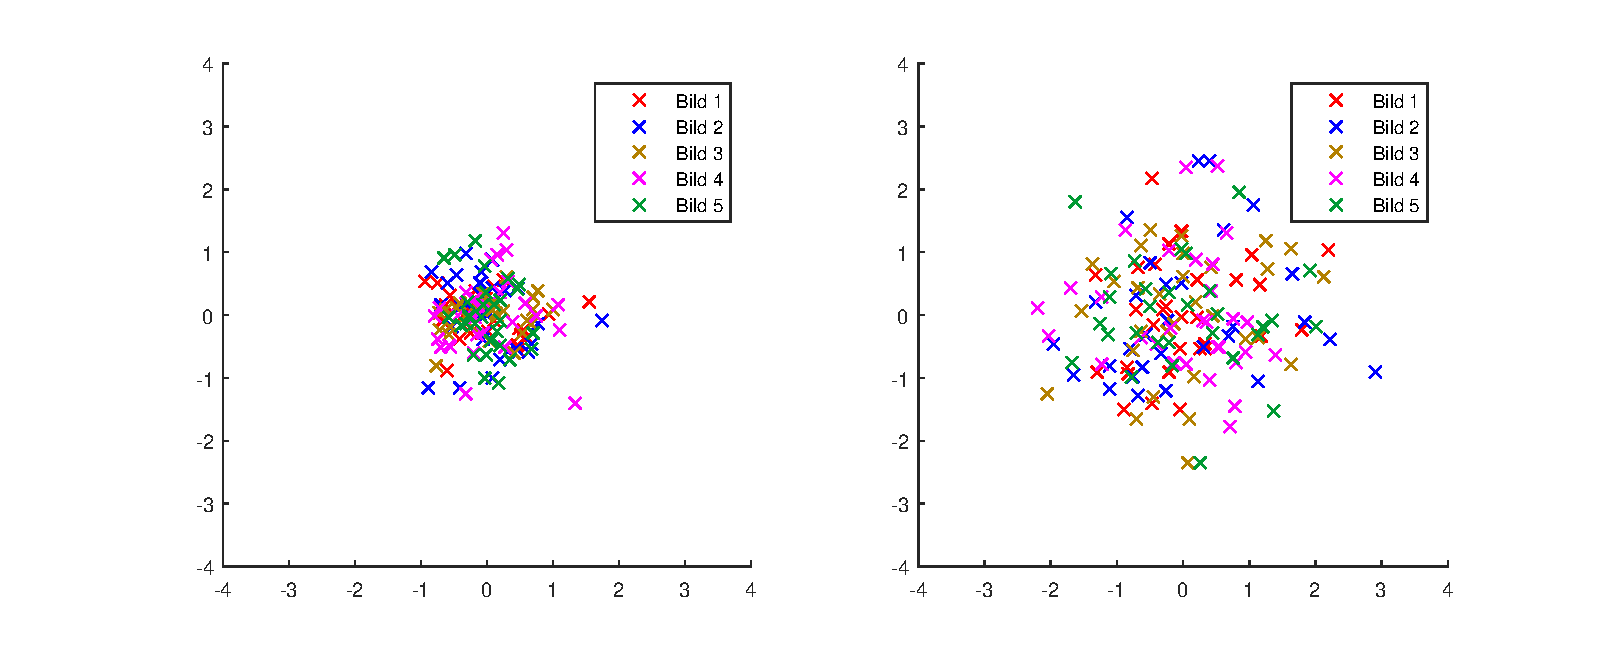
\includegraphics[width=\textwidth]{images/reprojectionErrorReverse.eps}
	\caption{Einfluss der intrinsischen Kalibrierung auf den Reprojektionsfehler}
	\label{fig:influenceCalib}
\end{figure}


Es ist klar zu erkennen, dass der Reprojektionsfehler bei den Bildern ohne intrinsische Kamerakalibrierung wesentlich größer ist. Der starke Einfluss kommt unter Anderem daher, dass wir eine Weitwinkelkamera mit starker tonnenförmiger Verzerrung eingesetzt haben. Ohne eine Modellierung der Linsenverzerrungen weichen die Abstände zwischen den Sample-Positionen stark von der Realität ab. Die Projektionsmatrix wird mit fehlerhaften Daten bestimmt. Die eigentlichen Sample-Positionen auf dem entzerrten Bild, werden also nicht korrekt auf die Sample-Positionen im Ursprungsbild abgebildet. 

\section{Einfluss der Rotation der Kamera}
Um den Einfluss der Rotation der Kamera untersuchen zu können, wurde der Kegel mit Kalibrierungsmuster gerendert, da die Kameraposition dann exakt bekannt ist und äußere Faktoren wie Lichtverhältnisse und inhomogene Hintergründe kontrolliert werden können. In Abbildung \ref{fig:blender} ist bei zwei unterschiedlichen Winkeln der gerenderte Kegel zu sehen. 

\begin{figure}[!htb]
	\centering
	\begin{subfigure}{.5\textwidth}
		\centering
		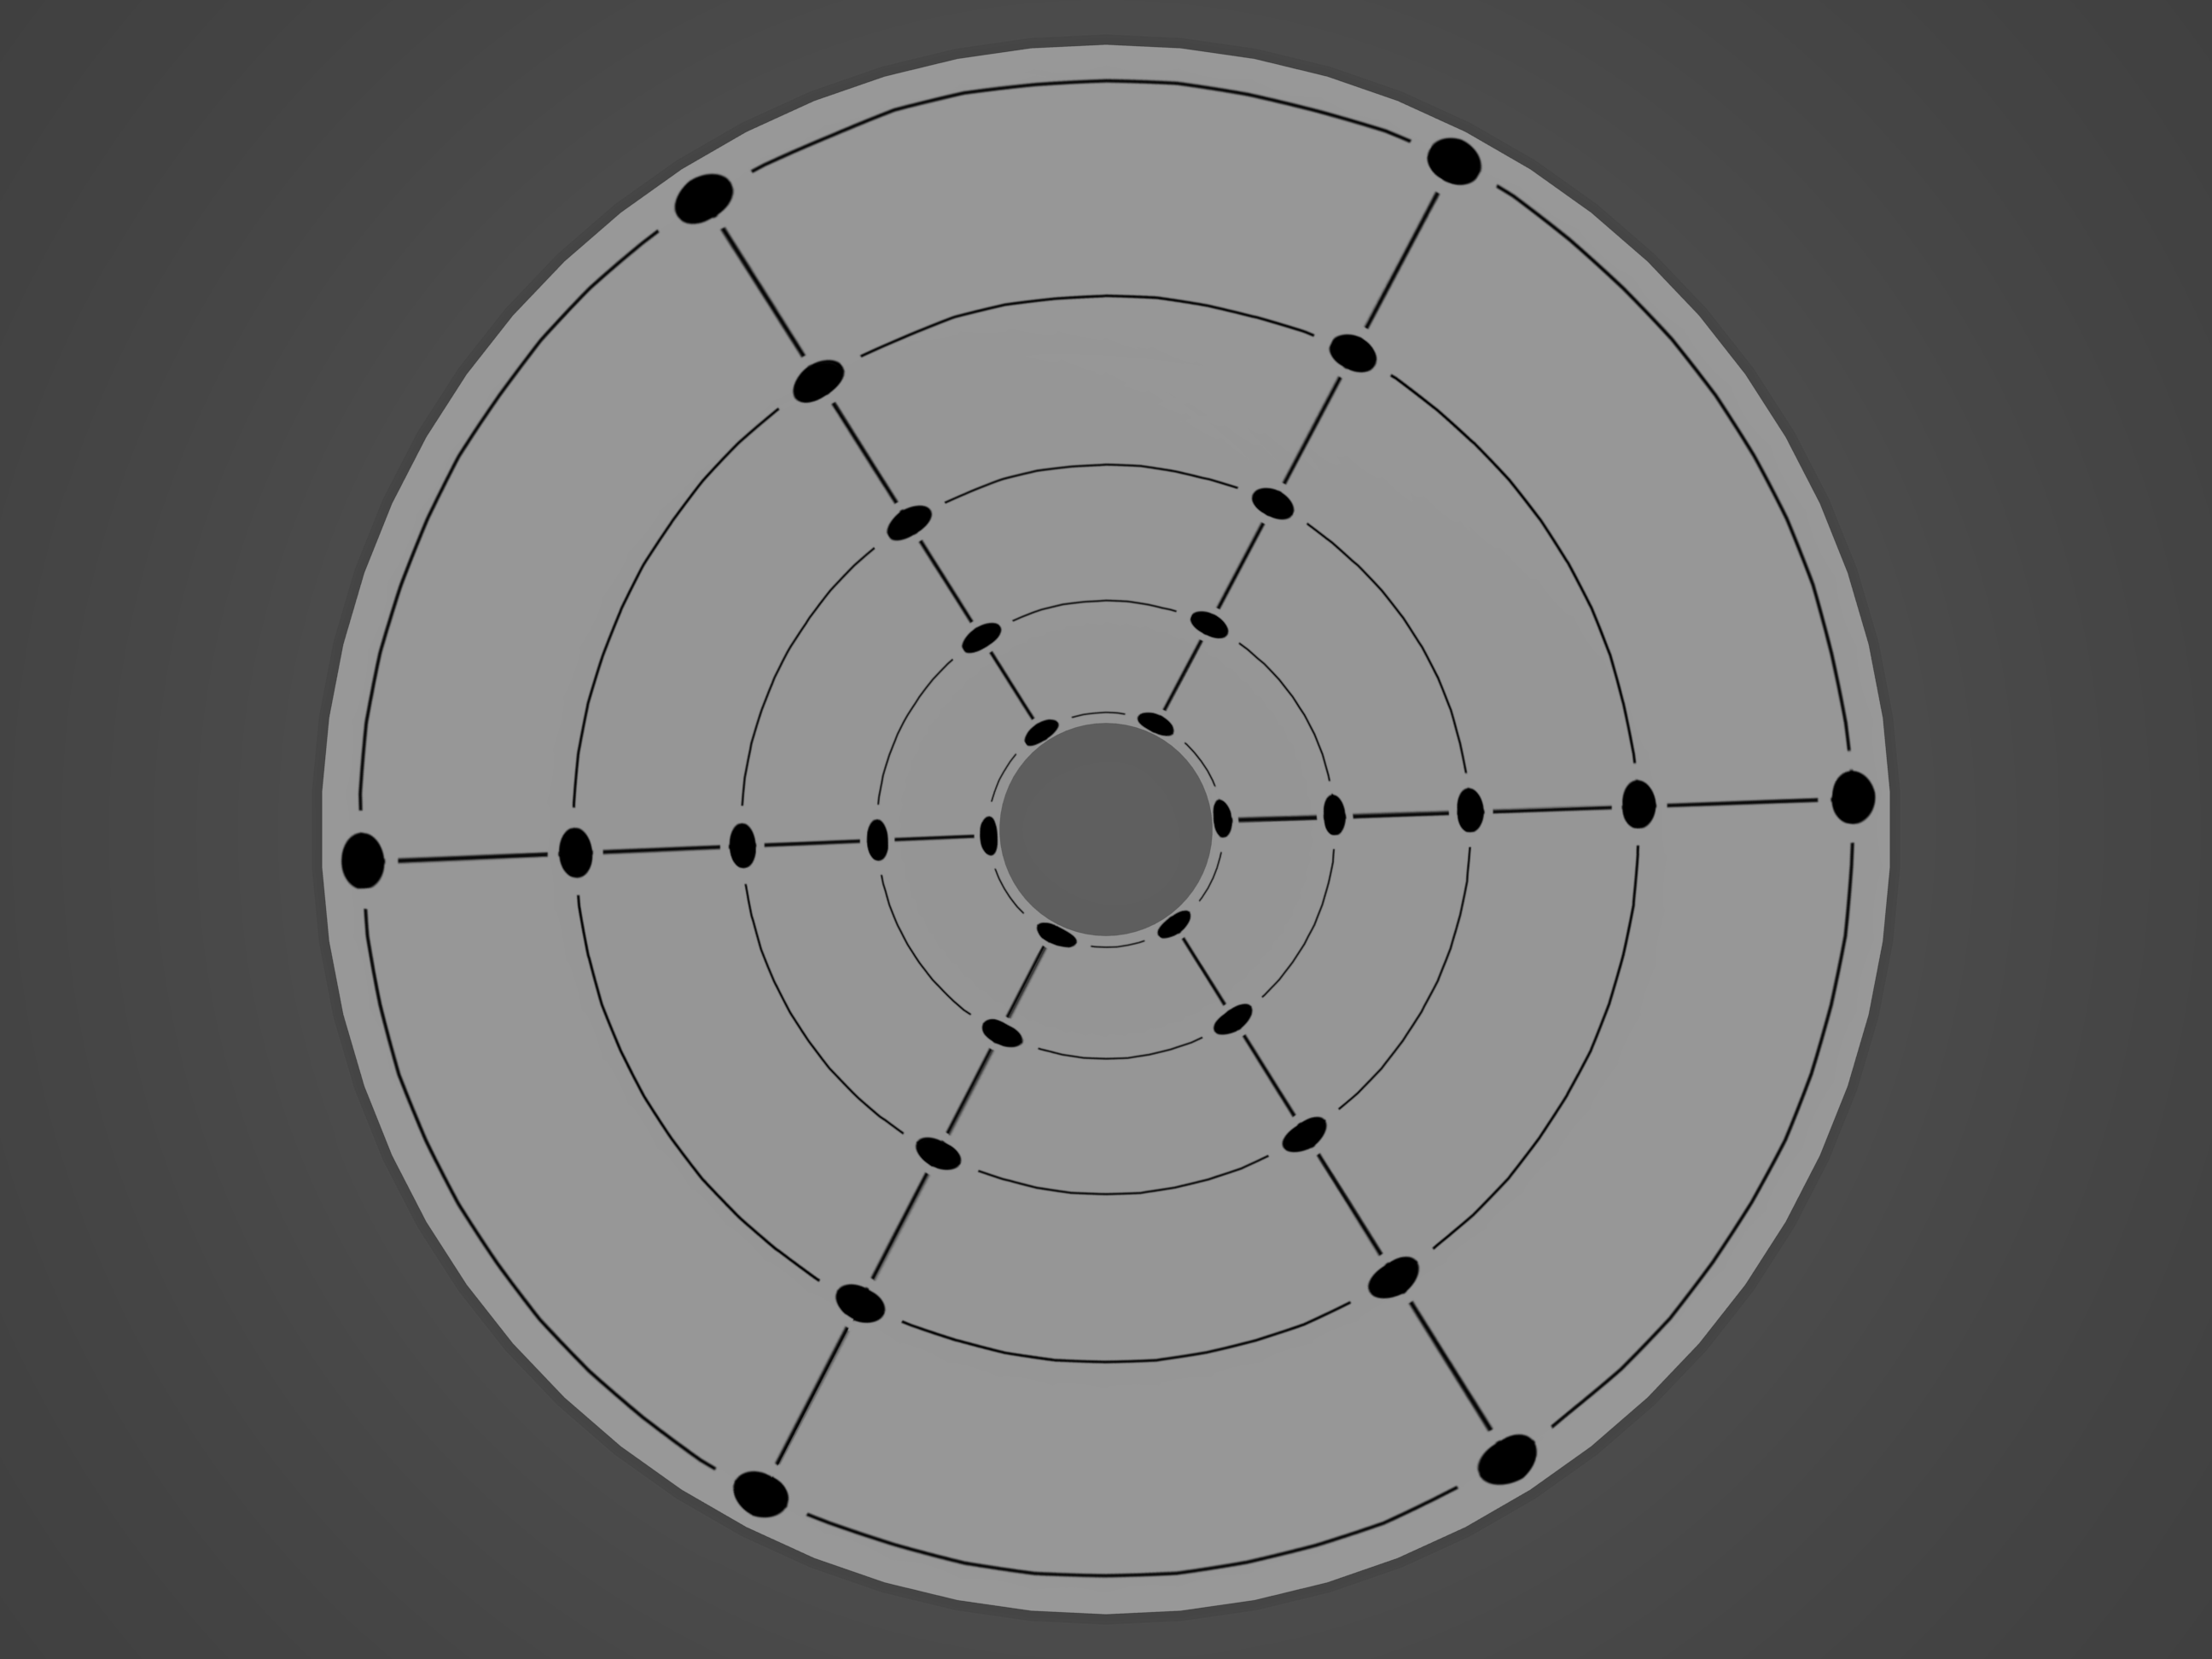
\includegraphics[width=.9\textwidth]{images/blender0.png}
		\caption{bei 0°}
	\end{subfigure}%
	\begin{subfigure}{.5\textwidth}
		\centering
		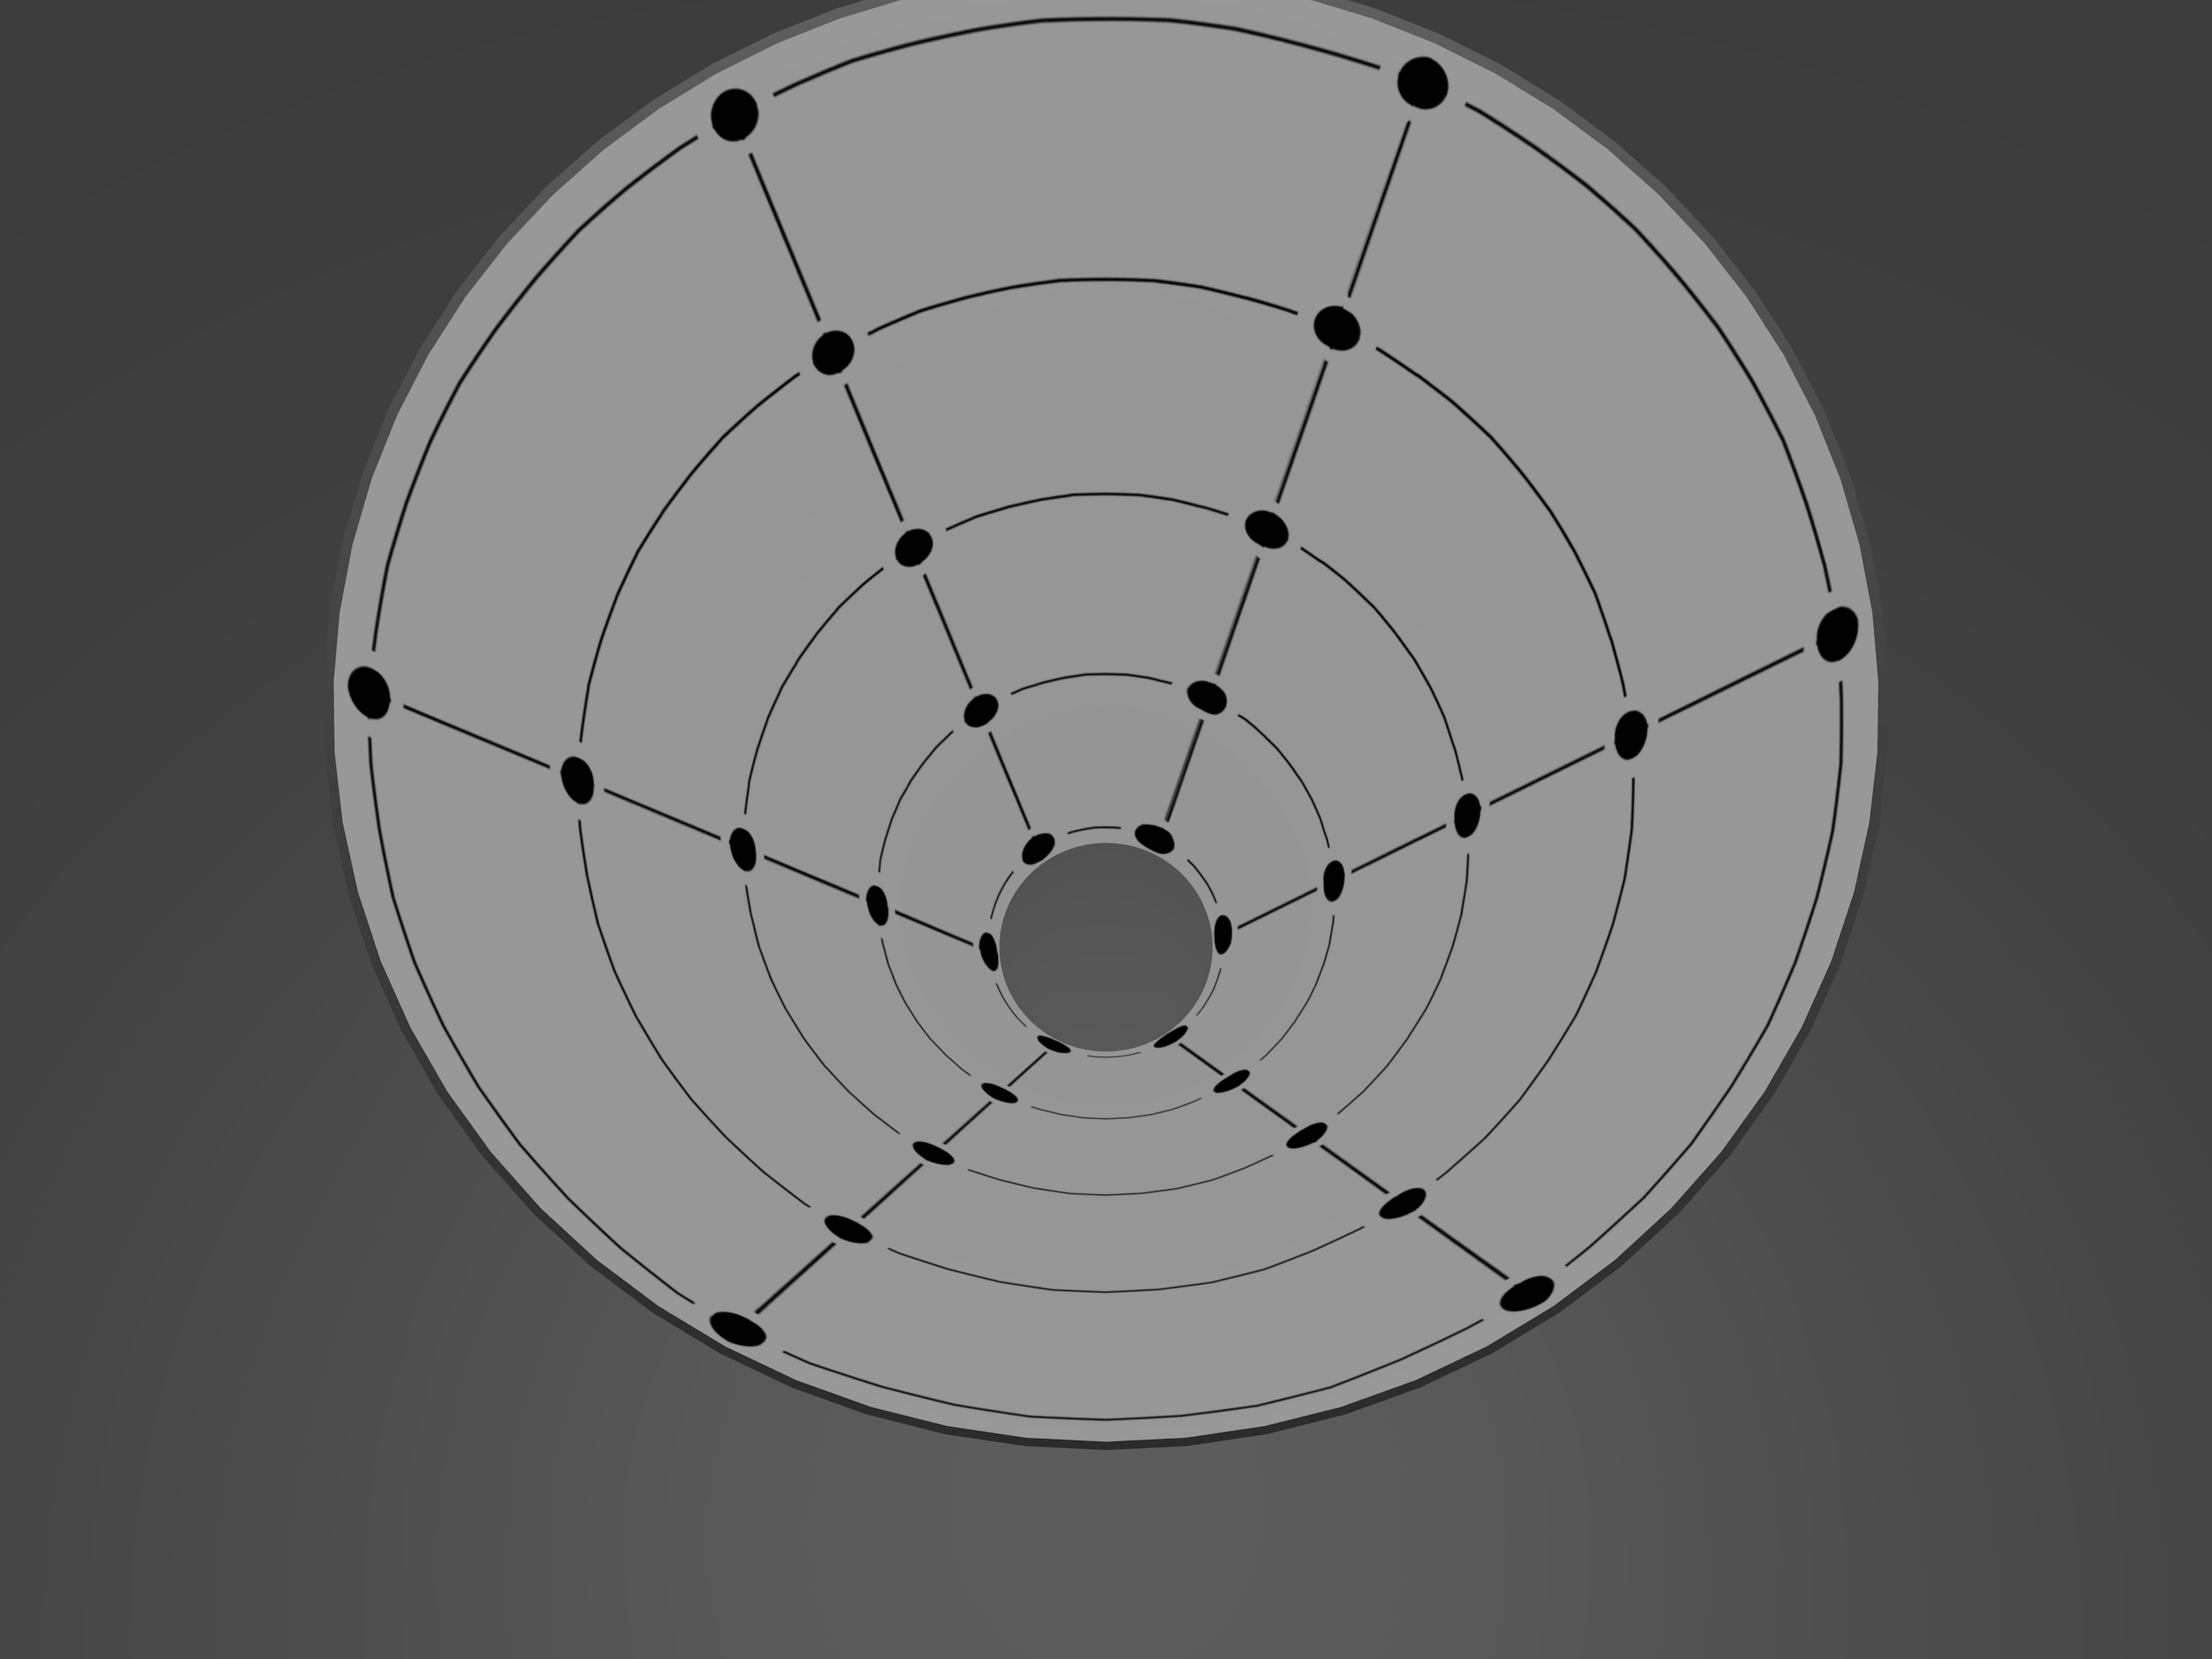
\includegraphics[width=.9\textwidth]{images/blender12.png}
		\caption{bei 12°}
	\end{subfigure}
	\label{fig:blender}
	\caption{gerendeter Kegel mit Kalibrierungsmuster in Blender aus verschiedenen Blickrichtungen}
\end{figure}


Es werden anschließend Bilder erzeugt, in denen in 1° Schritten die Kamera von 0° bis 12° um die $x$-Achse rotiert wird. Für jedes dieser Bilder wird anschließend eine Rückwärtsentfaltung durchgeführt und der durchschnittliche Reprojektionsfehler ermittelt. Abbildung \ref{fig:influenceRot} zeigt, dass der Reprojektionsfehler relativ rotationsinvariant ist bei einem durchschnittlichen . Ab einem Winkel von  13°, werden die Samples teilweise vom Blob-Detektor nicht mehr erkannt (bei 13° und 14° werden zwei nicht erkannt, bei 15° und 16° jeweiles vier) und mussten per Hand markiert werden. Ab einem Winkel von 16° sind die Abstände zischen den Kreislinien so klein, dass die Ellipsendetektion fehlschlägt. 


\begin{figure}[!htb]
	\centering
	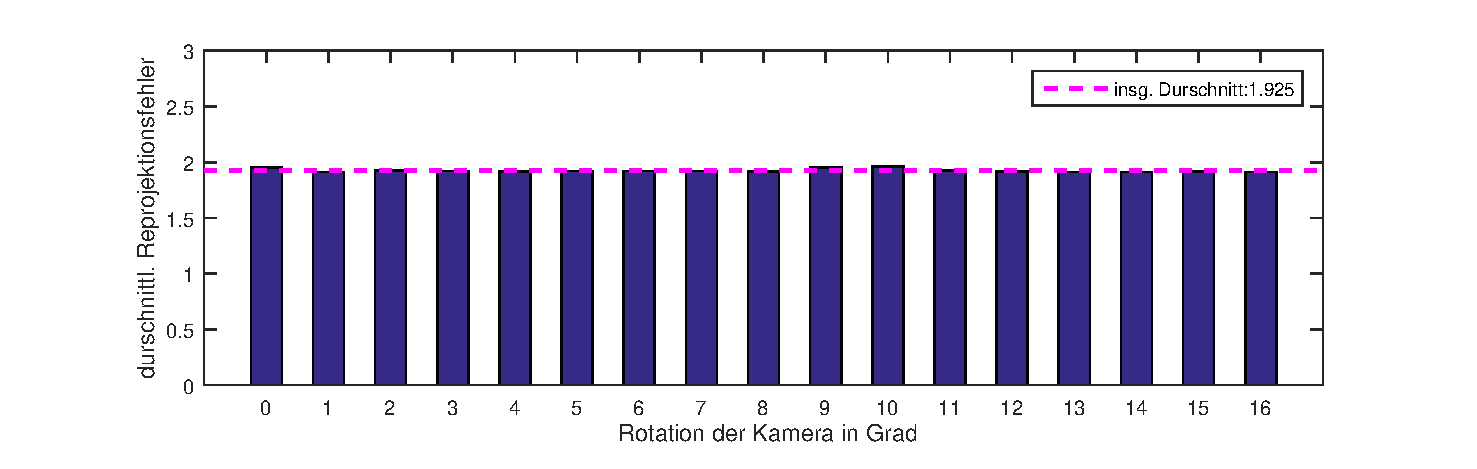
\includegraphics[width=\textwidth]{images/reprojectionErrorDeg2.eps}
	\caption{Einfluss der Rotation der Kamera}
	\label{fig:influenceRot}
\end{figure}


\section{Laufzeit der Entfaltung}
Durch den Kalibrierungsprozess erhalten wir zwei Abbildungsmatrizen (siehe Kapitel \ref{ch:implementation}), mit denen wir anschließend eine Reihe von Bildern entzerren möchten. Wir untersuchen dabei die Laufzeit pro gewählter Auflösung, in 50er Schritten, und ermitteln jeweils die Laufzeit gemittelt über 200 Bilder. Untersucht wird die Laufzeit mit bikubischer, sowie mit (bi-) linearer Interpolation. 

Im Gegensatz zu linearer Interpolation, werden bei bikubischer Interpolation , 16 Nachbarn statt vier betrachtet und mittels (stückweise stetiger) Polynome interpoliert. Der Aufwand bei der bikubischen Interpolation ist wesentlich größer, es entstehen aber weniger Artefakte \cite{Keys1981}.

Wie in Abbildung \ref{fig:influenceRes2} zu sehen, wächst die Laufzeit bei beiden Verfahren quadratisch mit der Auflösung der Seitenhöhe. Die Laufzeit des Verfahrens mittels bikubischer Interpolation wächst dabei um einen Faktor von $1.35$ schneller, als das Verfahren mittels linearer Interpolation.

\begin{figure}[!htb]
	\centering
	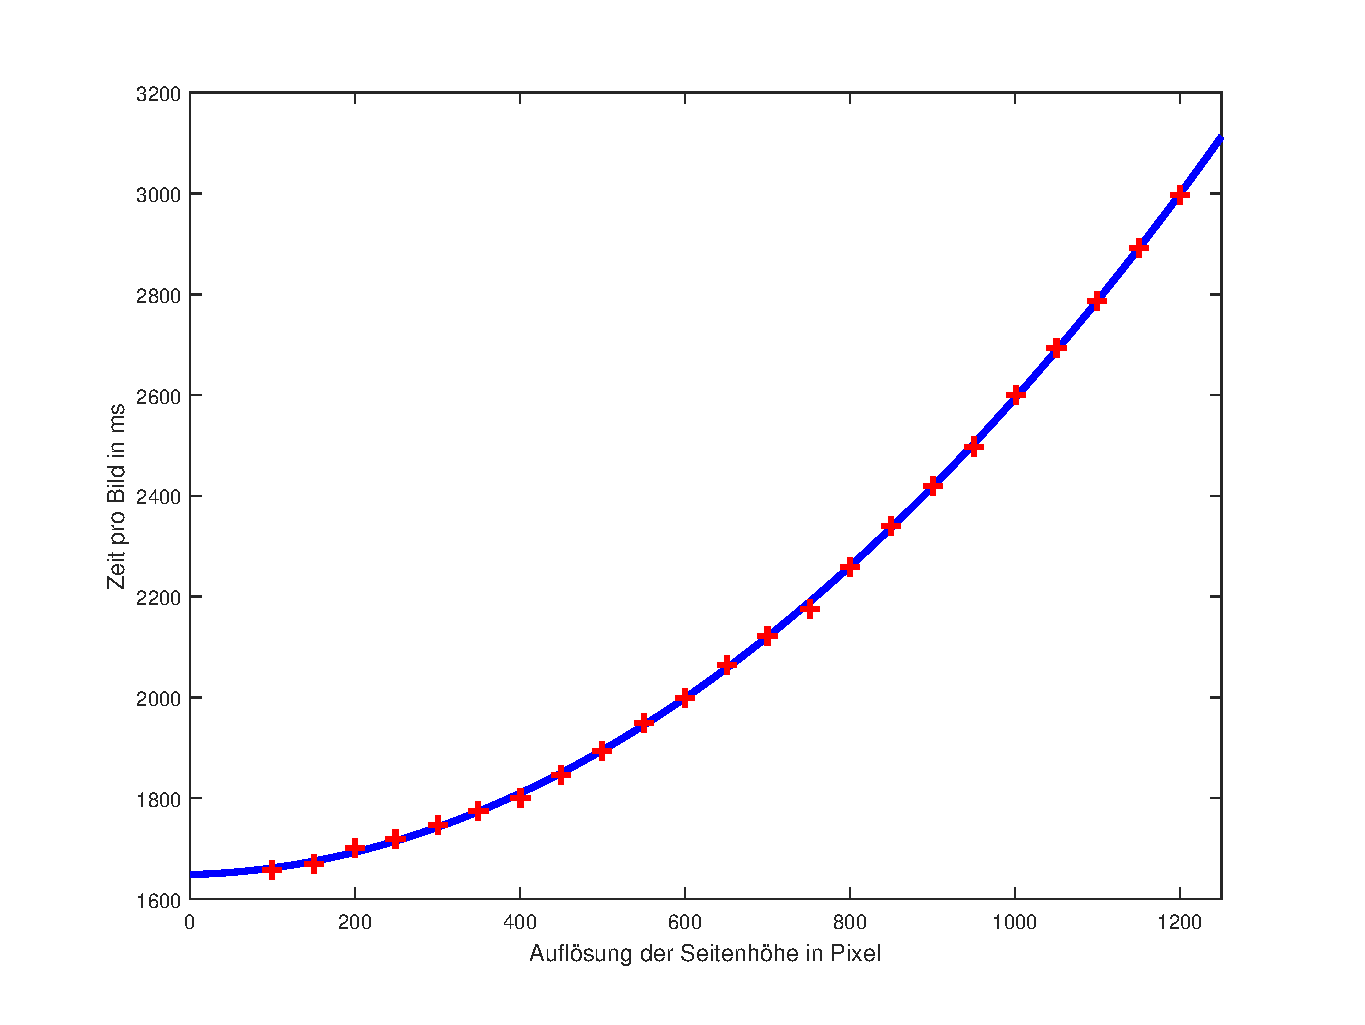
\includegraphics[width=0.8\textwidth]{images/runningTimePerSlantheight.eps}
	\caption{Einfluss der Ausgabeauflösung auf die Laufzeit der Entfaltung}
	\label{fig:influenceRes2}
\end{figure}

\section{Evaluierung der Ellipsendetektion mittels Deformable Templates}
Das Problem bei der Ellipsendetektion mittels {Deformable Templates ist, dass die Energiefunktion, auch nach starker Glättung des Kanten- und Kantenrichtungsbilds, schnell in kleine lokale Minima läuft, obwohl ein wesentlicher stärkeres Minimum in näherer Umgebung wäre. 

In Abbildung \ref{fig:deformable} sieht man beispielhaft einen Auschnitt der Energiefunktion, wobei in diesem Fall zwecks Veranschaulichung nur die Haupt- und Nebenachse der Ellipse variable sind. Das Zentrum bleibt das Zentrum des Bildes und der Winkel $\theta$ ist konstant null. Trotz dieser Einschränkungen lässt sich gut erkennen, dass circa bei $a = b = 350$ ein starkes Minimum liegt. Es gibt jedoch neben diesem Minimum in näherer Umgebung kleine irrelevante Minima, wie beispielsweise in $(350, 260)$. Solche "`Becken"' (in rot markiert) erschweren die Detektion erheblich.

Darüber hinaus muss für ein robustes und effizientes Optimierungsverfahren der Gradient und im besten Fall sogar die Hesse-Matrix der zu minimierenden Funktion zur Verfügung gestellt werden.  Jede Ableitung des Kanten- und Kantenorientierungsbilds bringt Unstetigkeitsstellen mit sich. Mit einer zu starke Glättung, geht jedoch viel Informationsverlust einher. Auch das korrekte Einstellen der Einflussparameter $\alpha,\beta$ und $\gamma$ (siehe Gleichung \ref{eq:deformTerms}) hat sich als große Herausforderung erwiesen. \todo{ist schon eher Fazit}.


\begin{figure}[!htb]
	\centering
	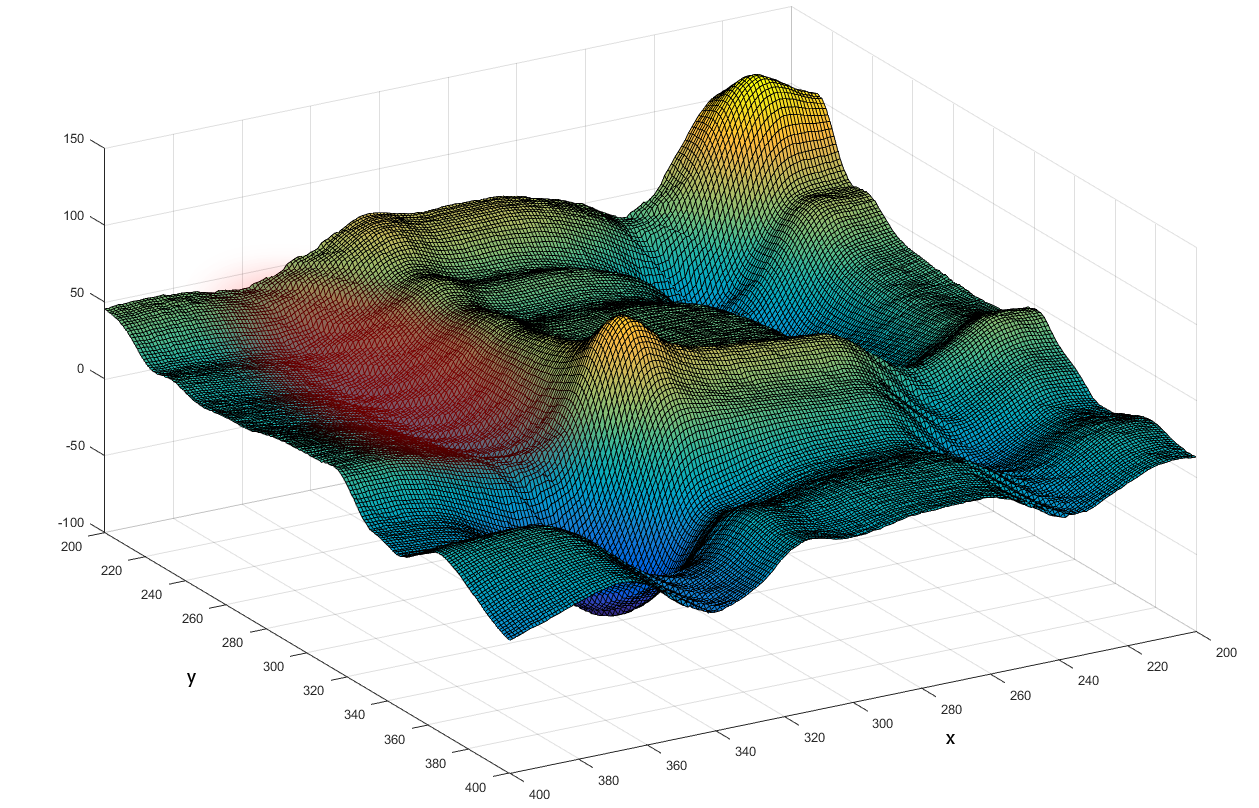
\includegraphics[scale=.4]{images/deformableHighlighted.png}
	\caption{Deformable Templates: Ausschnitt der Energiefunktion für variable Haupt- und Nebenachse}
	\label{fig:deformable}
\end{figure}


\section{Evaluierung der Ellipsendetektion mittels RANSAC}
Die robuste Ellipsendetektion ist der wichtigste Schritt bei der Entzerrung. Bei beiden Verfahren werden die bestimmten Ellipsen genutzt um Korrespondenzen zwischen den Sample-Positionen und Punkten auf dem Kegel im Weltkoordinatensystem herzustellen. Bei der Vorwärtsentfaltung werden die Ellipsen darüber hinaus benötigt, um für die Pixel geeignete 3D-Koordinaten interpolieren zu können. Es ist also von großer Bedeutung wie gut die Ellipsendetektion mittels RANSAC funktioniert.  


\begin{figure}[!htb]
	\centering
	\begin{subfigure}{.5\textwidth}
		\centering
		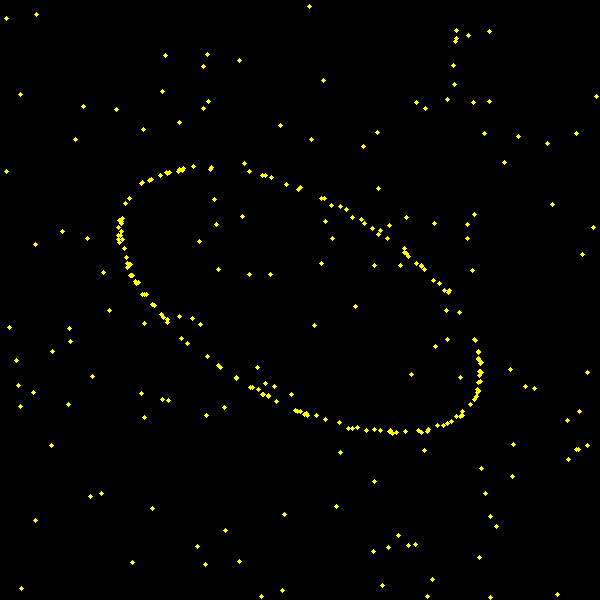
\includegraphics[width=.9\textwidth]{images/ransac50_0.png}
		\caption{gestörte Messdaten}
		\label{fig:uniformRansac1}
	\end{subfigure}%
	\begin{subfigure}{.5\textwidth}
		\centering
		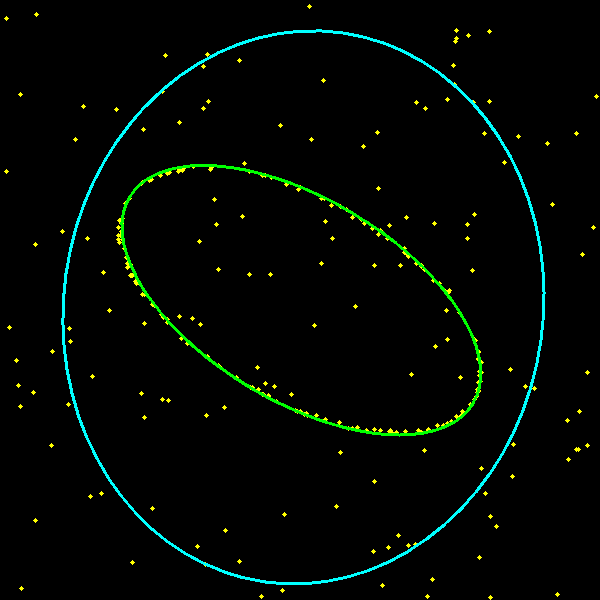
\includegraphics[width=.9\textwidth]{images/ransac50_1.png}
		\caption{detekt. Ellipsen: RANSAC (grün), LSQ (cyan)}
		\label{fig:uniformRansac2}
	\end{subfigure}
	\label{fig:uniformRansac}
	\caption{Vergleich RANSAC und LSQ bei gleichverteilten Ausreißern $\epsilon = 0.5, p = 0.99$}
\end{figure}

Wir betrachten zunächst, wie sich eine Gleichverteilung von Ausreißern auf die Schätzung der Ellipse auswirkt. Wie in Abbildung \ref{fig:uniformRansac1} erzeugen wird dazu zunächst eine Ellipse und bestimmen $500$ gleichverteilte Punkte auf der Ellipse. Anschließend erzeugen wir auf dem gesamten Bild gleichverteilt zu einem gegebenen Fehleranteil Ausreißer. Wir inkrementieren den Fehleranteil schrittweise von 0\% bis 60\% und vergleichen die Schätzungen durch Ransac und der Methoder der kleinsten Quadrate mit der eigentlichen Ellipse. Als Fehlermaß benutzen wir den Dice-Koeffizienten \cite{Dice1945}:

\[
	D = \frac{2\abs{A\cap B}}{\abs{A} + \abs{B}} \in [0, 1]
\]

für zwei Mengen $A$ und $B$ mit einem Wert von eins für eine perfekte Übereinstimmung $(A = B)$ und einem Wert von null, falls $A\cap B = \emptyset$. Wir betrachten hierbei die Ellipsen als Mengen, wobei die Punkte in einer Ellipse die Element der Menge sind. Die Anzahl der Iterationen für RANSAC kann in jedem Schritt berechnet werden mit Hilfe der Formel aus Kapitel \ref{s:ransac}.

In Abbildung \ref{fig:uniformEval} sieht man, dass der Dice-Koeffizient bei RANSAC konstant nahezu bei eins liegt. Das heißt, dass mittels RANSAC auch bei einem Fehleranteil von 60\% immer noch mit sehr großer Genauigkeit die Ellipse korrekt geschätzt wird. Bei der Methode der kleinsten Quadrate weicht die geschätzte Ellipse schon bei einem kleinen relativen Fehleranteil von 10\% stark von der korrekten Ellipse ab. 


\begin{figure}[!htb]
	\centering
	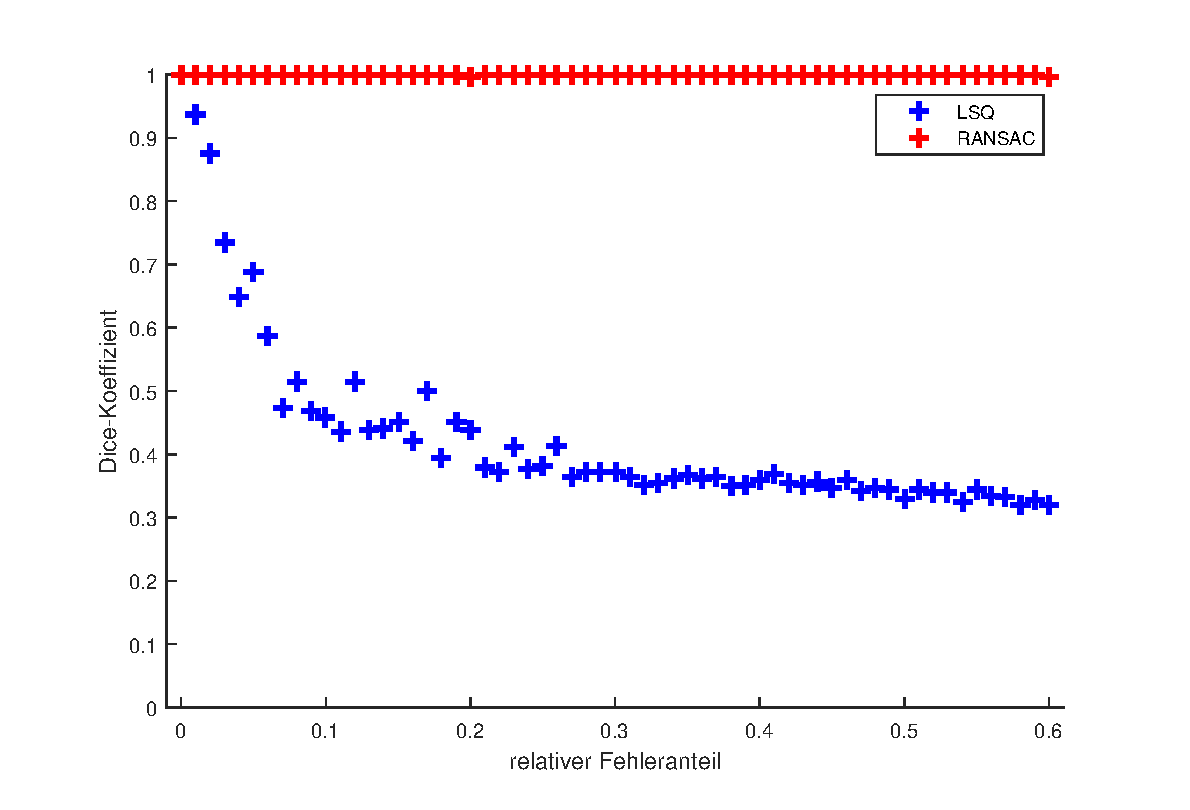
\includegraphics[width=\textwidth]{images/ransacEval0.eps}
	\caption{Vergleich von RANSAC und der Methode der kleisten Quadrate (LSQ) bei gleichverteilten Ausreißern}
	\label{fig:uniformEval}
\end{figure}

In unserem Verfahren ist eine Gleichverteilung der Ausreißer unwahrscheinlich. Viel wahrscheinlicher ist es, dass eine der nächst äußeren Ellipsen frühzeitig sichtbar wird (siehe Kapitel \ref{s:ellipseDetection}). 

\begin{figure}[!htb]
	\begin{subfigure}{.5\textwidth}
		\centering
		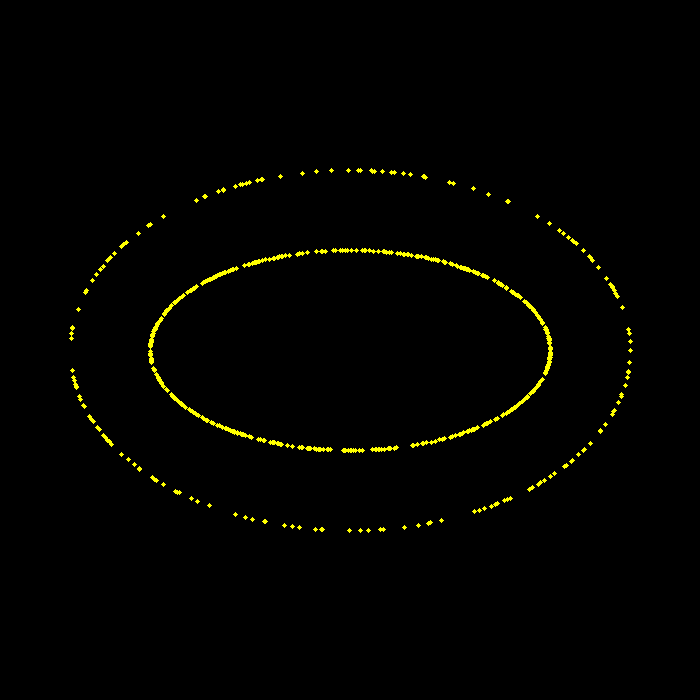
\includegraphics[width=.9\textwidth]{images/ransacShadow33_0.png}
		\caption{gestörte Messdaten}
		\label{fig:nonmUniformRansa1}
	\end{subfigure}%
	\begin{subfigure}{.5\textwidth}
		\centering
		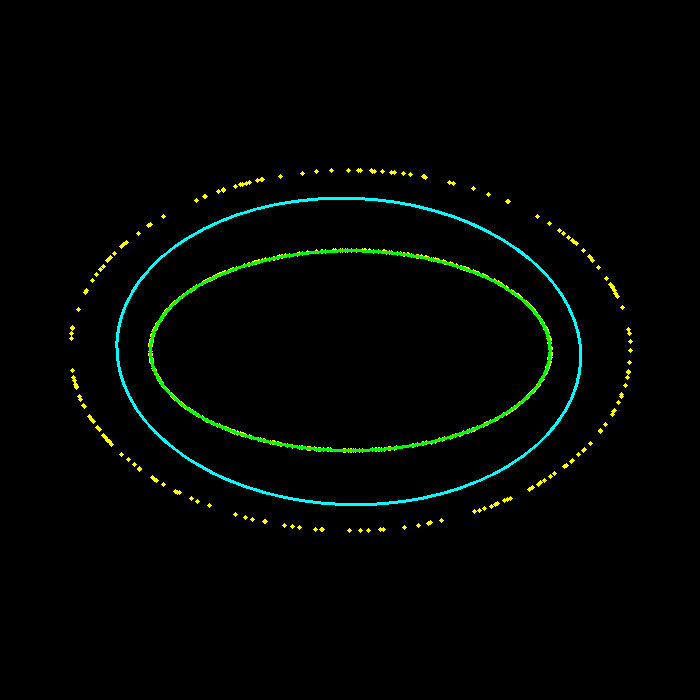
\includegraphics[width=.9\textwidth]{images/ransacShadow33_1.png}
		\caption{detekt. Ellipsen: RANSAC (grün), LSQ (cyan)}
		\label{fig:nonmUniformRansac2}
	\end{subfigure}
	\caption{Vergleich RANSAC und LSQ bei Schattenellipsen mit $p = 0.99$ und $\epsilon = 0.33$}
	\label{fig:nonmUniformRansac}
\end{figure}


\begin{figure}[!htb]
	\begin{subfigure}{.8\textwidth}
		\centering
		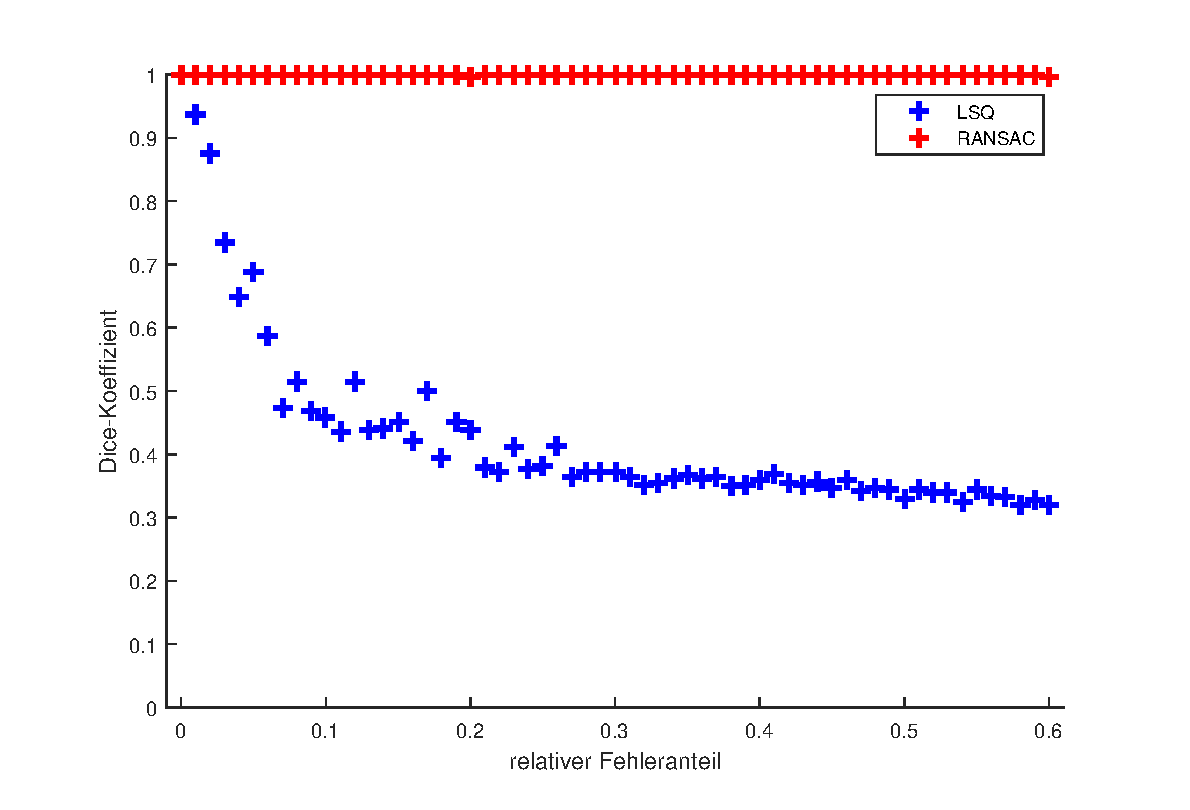
\includegraphics[width=\textwidth]{images/ransacEval0.eps}
		\caption{gestörte Messdaten}
	\end{subfigure}
	\begin{subfigure}{.8\textwidth}
		\centering
		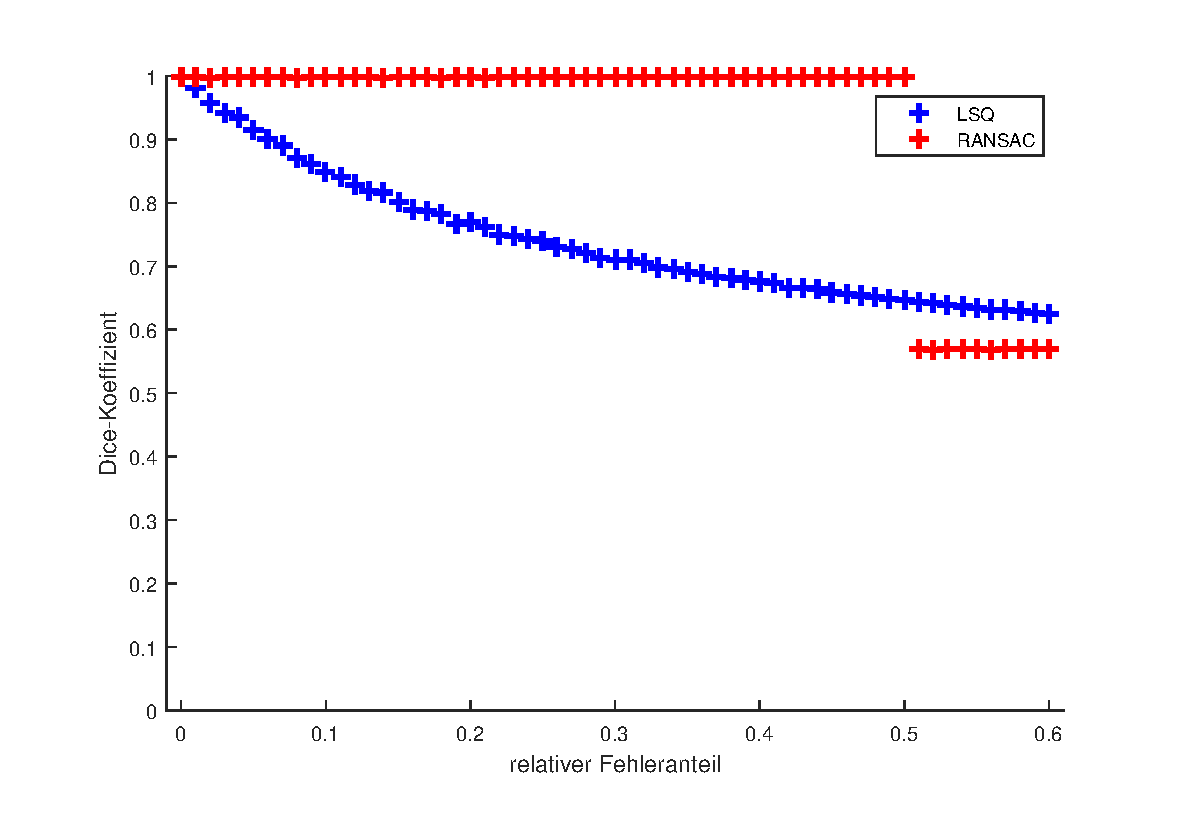
\includegraphics[width=\textwidth]{images/ransacEval1.eps}
		\caption{detekt. Ellipsen: RANSAC (grün), LSQ (cyan)}
	\end{subfigure}
	\caption{Vergleich RANSAC und LSQ bei Schattenellipsen mit $p = 0.99$ und $\epsilon = 0.4$}
	\label{fig:blubbs}
\end{figure}























